\section{Abbild erstellen}
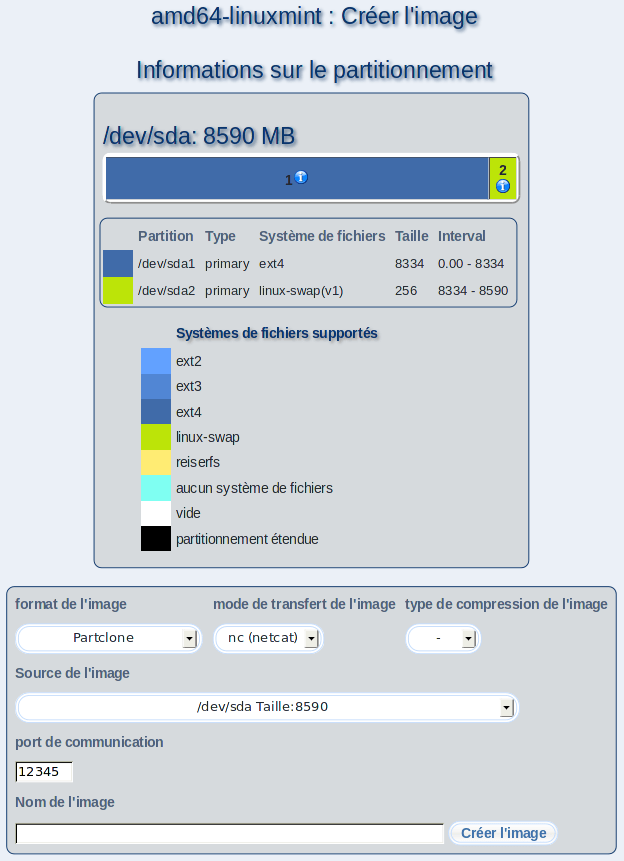
\includegraphics[scale=0.4]{/mdk/doc/manual/screenshots/de/client_createImage.png} \\
Mit diesem Dialog k�nnen Sie Dateiabbilder von Partitionen oder ganzen Laufwerken eines Clients erstellen, die Sie anschlie�end zum Installieren von anderen Clients nutzen k�nnen. W�hlen Sie dazu das gew�nschte Abbilddateiformat, den �bertragungsmodus und die Abbildkompression aus. Je nach Abbilddateiformat m�ssen Sie bei \textit{"Abbildquelle"} zus�tzliche Angaben machen, z.B. die Partition oder das komplette Laufwerk, das in der Abbilddatei gespeichert werden soll.\\
W�hlen Sie dann einen Namen f�r die Datei und tragen ihn unter \textit{"Abbildname"} ein. Klicken Sie anschlie�end auf \textit{"Abbild erstellen"}.\\
\subsection{Hinweis zu den Abbilddateien}
Die Dateien werden im Verzeichnis \textbf{/m23/data+scripts/clientImages} abgelegt und k�nnen in verschiedenen Formaten und mit anderen Verfahren komprimiert werden, sind aber immer nach dem gleichen Dateinamenschema aufgebaut: $\langle$Abbildname$\rangle$$\langle$Gr��e des entpackten Abbildes in Bytes$\rangle$$\langle$Abbildformat$\rangle$$\langle$Kompression$\rangle$\\
Hierbei kann das Abbildformat folgendes sein:\\
\begin{itemize}
\item \textbf{dd}: Speichert die kompletten Daten einer Partition oder Festplatte\\
\end{itemize}
F�r die Kompression sind folgende Werte g�ltig:\\
\begin{itemize}
\item  (keine Kompressionsendung): Die Abbilddatei ist nicht komprimiert.\\
\item \textbf{gz}: Komprimiert mit dem Programm gzip.\\
\item \textbf{bz2}: Komprimiert mit dem Programm bzip2 und komprimiert meist st�rker.\\
\end{itemize}
\subsection{Hinweis zum �bertragungs-Port}
F�r den �bertragungsmodus m�ssen Sie zus�tzlich einen Netzwerk-Port angeben, der auf Client- und Serverseite verwendet werden kann und nicht durch eine Firewall etc. geblockt ist. M�chten Sie mehrere Abbilder gleichzeitig erstellen, so m�ssen Sie unterschiedliche Ports w�hlen.\\
